\chapter{Studi Literatur}
\label{chapter:studi-literatur}

\section{Dasar Teori}
\label{sec:dasar-teori}
Subbab dasar teori merupakan subbab yang akan memberikan pengenalan
terhadap permasalahan yang akan dihadapi. Subbab ini juga akan memberikan konteks dan keterangan lebih lanjut mengenai teknologi-teknologi yang akan digunakan atau dipertimbangkan sebagai alternatif solusi dari permasalahan yang diangkat. Berikut merupakan landasan teori yang akan digunakan dalam penelitian ini.

\subsection{Pemrosesan Dokumen Finansial}
\label{subsec:pemrosesan-dokumen-finansial}

Dokumen struk pembayaran memegang peranan penting dalam pengelolaan
keuangan baik individu maupun institusi. Proses ekstraksi data dari dokumen-dokumen ini sering kali menghadapi tantangan yang signifikan, termasuk keanekaragaman tata letak, kualitas gambar yang bervariasi, dan kebutuhan untuk
mengekstrak informasi dengan akurasi tinggi. Sebagai contoh, elemen-elemen penting seperti total harga, tanggal transaksi, dan nomor rekening sering kali tersebar di berbagai posisi dalam dokumen yang berbeda, sehingga membuat ekstraksi data secara manual menjadi lambat dan rentan terhadap kesalahan.

Teknologi yang umumnya dapat digunakan untuk menanggulangi masalah ini adalah \cv{}, salah satunya \ocr. Secara tradisional, \ocr{} digunakan untuk mengonversi teks dalam gambar menjadi format digital yang dapat diproses lebih lanjut. Namun, OCR memiliki
keterbatasan, terutama dalam menangani dokumen dengan kualitas gambar rendah atau format teks yang tidak standar. Selain itu, ketergantungan pada OCR dapat meningkatkan kompleksitas dan biaya pemrosesan \parencite{kim2021donut}.

\dlfl{} memiliki berbagai jenis algoritma dan model yang mendukung pengembangan sistem tersebut. \dl{} merupakan cabang \ml{} yang memanfaatkan jaringan saraf tiruan berlapis untuk mengenali pola kompleks dalam data, termasuk dokumen finansial. Salah satu model yang umum digunakan adalah \cnn. \cnn{} dirancang untuk memproses data berbentuk gambar dengan mendeteksi fitur lokal seperti teks, garis, atau elemen visual lainnya sehingga \linebreak cocok untuk ekstraksi data dari dokumen. Namun, \cnn{} terbatas dalam memahami hubungan global antar
elemen dalam dokumen sehingga \transformer{} hadir sebagai solusi yang lebih canggih \parencite{alzubaidi2021review}.

Dengan mekanisme \attention-nya, \transformer{}, seperti LayoutLM dan
Donut, mampu menangkap hubungan kontekstual antar elemen secara global. Hal ini membuat penggunaan \transformer{} dengan struktur kompleks dan informasi
tersebar. \transformer{} memberikan pendekatan yang kuat untuk memastikan akurasi dan efisiensi dalam pemrosesan dokumen finansial.

\subsection{\emph{Deep Learning}}
\label{subsec:dl}

\dlfl{} adalah cabang dari \ml{} yang menggunakan \annfull{} dengan banyak lapisan untuk mempelajari representasi data yang kompleks. Deep Learning memungkinkan komputer untuk menganalisis data tidak terstruktur, seperti teks, gambar, audio, dan video dengan tingkat akurasi yang sangat tinggi. Model-model \dl{} belajar dengan cara memproses data melalui lapisan-lapisan neuron atau saraf yang dirancang untuk mengekstrak fitur-fitur penting, baik yang eksplisit maupun tersembunyi \parencite{Goodfellow-et-al-2016}. 

Terdapat beberapa model dan arsitektur yang dapat digunakan dalam \dl. Setiap model tersebut ditujukan untuk memenuhi kasus yang berbeda-beda. Berikut adalah arsitektur dan model yang relevan dengan kasus ekstraksi data dari dokumen finansial.

\subsubsection {\cnn\--\transformer{}}
\cnn{} dan \transformer{} adalah dua metode yang dapat digunakan secara terpisah atau bersama untuk menangani data visual. \cnn{} adalah salah satu jenis \MakeLowercase{{\nn{}}} yang sering digunakan pada data gambar. CNN bisa digunakan untuk mendeteksi dan mengenali fitur signifikan tanpa supervisi manusia pada gambar \parencite{alzubaidi2021review}. \transformer{} adalah sebuah arsitektur \MakeLowercase{\nn{}} yang meng-\emph{encode} data menjadi fitur-fitur melalui mekanisme \attention. \transformer{} membagi gambar menjadi beberapa \patch{} dan mengkalkulasi representasi hubungan antar \patch{} tersebut \parencite{han2021transformer}. 

\subsubsection{\crnnfull}
\crnn{} adalah kombinasi dari \cnn{} dan \rnn{} yang merupakan dua model yang paling sering digunakan. \cnn{} digunakan pada tahap awal untuk mengekstrak fitur visual dan gambar. Hasil dari implementasi \cnn{} akan digunakan oleh model \rnn{} sebagai data input untuk menangkap hubungan antar elemen teks, seperti urutan huruf dalam kata atau angka dalam bilangan \parencite{wang2019convolutional}. \crnn{} telah diaplikasikan pada klasifikasi musik, audio, dan klasifikasi data serta teks yang bersifat \emph{hyperspectral}.

\subsubsection{Model \objectdetection}
Model \objectdetection{} adalah salah satu model dalam \dl{} yang digunakan untuk mendeteksi dan mengenali objek-objek tertentu dalam sebuah gambar atau dokumen, termasuk elemen-elemen seperti teks, tabel, atau simbol pada dokumen finansial. Dua jenis utama model \objectdetection{} yang sering digunakan adalah \yolofull{} dan \rcnnfull{}.
	\begin{enumerate}
		\item \yolo~\\
		\yolo{} adalah model \objectdetection{} yang dirancang untuk kecepatan tinggi dan efisiensi. \yolo{} memproses seluruh gambar dalam satu tahap dengan membagi gambar menjadi \grid{}, kemudian memprediksi bounding box dan kelas objek secara bersamaan di setiap \grid{} \parencite{diwan2023object}. Model ini terkenal karena kecepatannya. Dengan kecepatan tersebut, model ini cocok untuk aplikasi \emph{real-time} meskipun memiliki kompromi dalam akurasi untuk objek kecil atau yang saling berdekatan.
		\item \rcnn~\\
		\rcnn{} menggunakan pendekatan dua tahap. \rcnn{} menghasilkan proposal wilayah yang berpotensi mengandung objek pada tahap pertama. Pada tahap kedua, setiap proposal dianalisis lebih mendalam menggunakan \cnn{} untuk mengklasifikasikan objek dan memperbaiki bounding box. \rcnn{} dan variannya, yaitu Fast \rcnn{} dan Faster \rcnn{}, menawarkan akurasi tinggi walaupun memerlukan waktu komputasi yang lebih lama. Dengan sifat tersebut, model ini lebih cocok untuk aplikasi yang tidak membutuhkan deteksi \emph{real-time} \parencite{xie2021oriented}.
	\end{enumerate}

\subsection{\transformer}
\label{subsec:transformer}

\transformer{} adalah suatu jenis arsitektur jarigan yang baru dalam \dl. Arsitektur ini digunakan untuk mentransformasi sebuah deretan data menjadi sesuatu dengan karakteristik, seperti panjang atau format, yang berbeda. \transformer{} tidak menggunakan lapisan rekursif (\rnn) atau konvolusi (\cnn). \transformer{} menggunakan mekanisme \selfattention{} yang memungkinkannya untuk memahami hubungan antar elemen dalam sebuah deretan atau urutan (\sequence). Tidak seperti pada \rnn{}, mekanisme \selfattention{} tidak perlu memperhatikan jarak antar elemen. Mekanisme ini membuat \transformer{} menjadi sangat efisien untuk memproses data sekuensial. \transformer{} banyak digunakan pada proses penerjemahan bahasa, rangkuman teks, dan pengenalan suara.

\transformer{} terdiri atas dua komponen utama, yaitu \encoder{} dan \decoder. \encoderfl{} bertugas untuk membaca dan memproses \sequence{} masukan, sementara \decoder{} menghasilkan \sequence{} keluaran berdasarkan informasi dari \encoder. \encoderfl{} dan \decoder{} terdiri dari beberapa lapisan yang identik, dengan masing-masing memiliki dua sub-lapisan utama, yaitu \emph{multi-head attention} dan \emph{feed-forward network}.

\subsubsection{\mha}
Sublapisan ini menggunakan mekanisme \selfattention{} untuk memahami hubungan antar elemen dalam sebuah \sequence{}. Misalnya, dalam sebuah kalimat, mekanisme ini dapat mengenali bahwa kata "dia" merujuk pada "ibu" meskipun terdapat kata-kata lain di antaranya. \mha{} merupakan gabungan beberapa lapisan (\layer) \emph{Scaled Dot-Product Attention}, atau akan disingkat menjadi \attention. Perbandingan proses pada \mha{} dan \emph{Scaled Dot-Product Attention} dapat dilihat pada \autoref{fig:attention}
	\begin{figure}[htbp]
		\centering
		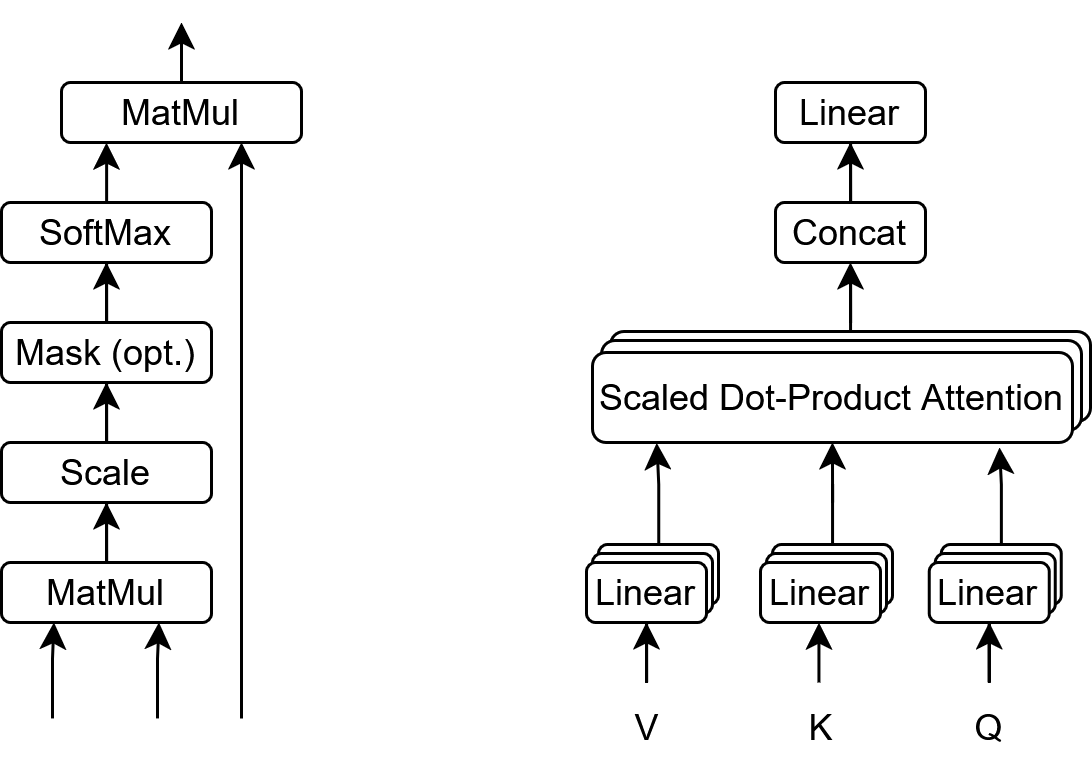
\includegraphics[width=.8\textwidth]{images/attentionmha.png}
		\caption{\emph{Scaled Dot-Product Attention} (kiri) dan \mha{} (kanan) yang merupakan beberapa \layer{} \attention{} berjalan paralel \parencite{vaswani2017attention}}
		\label{fig:attention}
	\end{figure}

$Q$ (\emph{Query}), $K$ (\emph{Key}), dan $V$ (\emph{Value}) adalah representasi vektor dari setiap elemen dalam sebuah \sequence. Simbol $d_k$ adalah dimensi dari vektor $K$ yang digunakan untuk menghasilkan perkalian \emph{dot-product} $QK^\mathsf{T}$ agar proses pelatihan tetap stabil. Fungsi Softmax kemudian mengubah skor tersebut menjadi bobot probabilistik untuk menentukan elemen yang paling relevan untuk diperhatikan.
\newpage
Perhitungan \attention{} dilakukan dengan formula seperti yang ditunjukkan pada persamaan \eqref{eq:attention-softmax} \parencite{vaswani2017attention} yang didefinisikan sebagai berikut.

\begin{equation}
	\label{eq:attention-softmax}
		\operatorname{Attention}(Q, K, V) = \operatorname{SoftMax}\left(\frac{QK^\mathsf{T}}{\sqrt{d_k}}\right)V
\end{equation}
\addcontentsline{loe}{myequations}{\protect\numberline{\theequation}Persamaan Softmax}

\subsubsection{\ffnfull}
Setelah \attention{} dihitung, informasi dari setiap elemen diproses melalui jaringan \emph{feed-forward} yang sama untuk setiap posisi dalam \sequence. Jaringan ini terdiri dari dua lapisan linier dengan fungsi aktivasi ReLU pada persamaan \eqref{eq:ffn} \parencite{vaswani2017attention}:

\begin{equation}
	\label{eq:ffn}
	\operatorname{FFN}(x) = \max(0, xW_1 + b_1)W_2 + b_2
\end{equation}
\addcontentsline{loe}{myequations}{\protect\numberline{\theequation}Fungsi Aktivasi ReLU pada \ffn}

\decoderfl{} memiliki perbedaan signifikan dibandingkan dengan \encoder. \encoderfl{} terdiri dari beberapa lapisan yang masing-masing memiliki mekanisme \selfattention{} dan FFN. Setiap elemen dalam \sequence{} dapat saling “memperhatikan”. \decoderfl{} memiliki lapisan tambahan, yaitu \encoder{}\--\decoder{} \attention. Lapisan ini memungkinkan \decoder{} untuk "memperhatikan" keluaran dari \encoder. \decoderfl{} memiliki mekanisme \emph{masking} untuk memastikan bahwa posisi saat ini hanya bergantung pada posisi sebelumnya.

\transformer{} memiliki keunggulan dibandingkan dengan metode konvensional pemrosesan sekuensial, seperti \rnn. \transformer{} tidak bergantung pada pemrosesan berurutan. \transformer{} dapat memproses seluruh urutan secara bersamaan dan membuat pelatihan jauh lebih cepat. Implementasi \transformer{} menunjukkan hasil terbaik di berbagai kasus dibandingkan dengan arsitektur lainnya.


\subsection{\donutfull}
\label{subsec:donut}

\donut{} adalah sebuah transformer yang tidak memerlukan penggunaan \ocr{} untuk melakukan pemahaman terhadap dokumen. Konsep utama \donut{} adalah pemetaan langsung dari gambar dokumen mentah menjadi hasil yang terstruktur dan melewati seluruh proses implementasi \ocr \parencite{kim2021donut}. \donut{} merupakan sebuah \emph{pre-trained model} yang menggunakan \emph{visual encoder Transformer}, yaitu \swin{} untuk melakukan ekstraksi fitur visual dari dokumen, dan \emph{text decoder Transformer}, yaitu \bartfull. Oleh karena itu, \donut{} tidak memiliki ketergantungan pada fungsionalitas \ocr{} sama sekali.

\textit{Pipeline} implementasi \transformer untuk pemahaman dokumen pada umumnya terlihat pada \autoref{fig:non-donut-pipeline}. \donut{} menyederhanakan pipeline ekstraksi data dokumen seperti terlihat pada \autoref{fig:donut-pipeline}. Dengan implementasi \textit{pipeline} yang lebih sederhana, proses ekstraksi data dokumen dapat diproses secara \ee{} melalui Donut tanpa perlu melewati fase \textit{pre-processing} dan \textit{post-processing} dari gambar \textit{input} dan \textit{output}.

\textit{Input} gambar akan diterima oleh \encoder, seperti \swin{} atau ResNet yang akan memecah gambar menjadi gambar-gambar kecil yang tidak saling bertumpuk. Hasil dari \encoder{} akan dikirimkan ke \decoder{} \transformer{} yang digunakan, seperti BART, untuk diproses menjadi \textit{output} berbentuk deretan teks. \textit{Output} yang dihasilkan akan dikonversi menjadi format \jsonfull.

\begin{figure}[htbp]
	\centering
	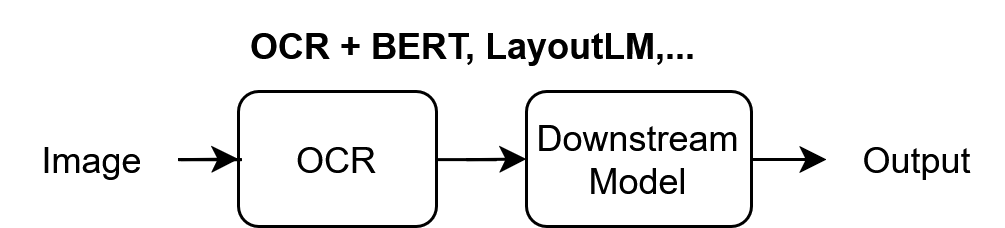
\includegraphics[width=0.8\textwidth]{images/non-donut-pipeline}
	\caption{\textit{Pipeline} sebelum implementasi \donut{} \parencite{kim2021donut}.}
	\label{fig:non-donut-pipeline}
\end{figure}

\begin{figure}[htbp]
	\centering
	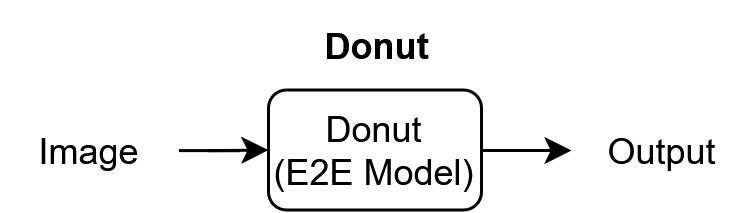
\includegraphics[width=0.8\textwidth]{images/donut-pipeline.png}
	\caption{\textit{Pipeline} setelah implementasi \donut{} \parencite{kim2021donut}.}
	\label{fig:donut-pipeline}
\end{figure}

\subsection{\swin}
\label{subsec:swin}

\swin{} adalah sebuah arsitektur \vitfull{} yang dirancang sebagai penopang dalam berbagai tugas \cv{} seperti klasifikasi gambar, deteksi objek, dan segmentasi semantik. Nama "Swin" berasal dari konsep
"\emph{Shifted Window}" yang menjadi elemen utama dalam desainnya. Tidak seperti \vit{} yang menggunakan metode \selfattention{} secara global
pada seluruh gambar, \swin{} memperkenalkan \selfattention{} berbasis \emph{local window} yang secara signifikan mengurangi kompleksitas komputasi \parencite{liu2021swin}. Perbedaan pendekatan \swin{} dan \vit{} dapat dilihat pada \autoref{fig:Swin-vs-ViT}. 

\begin{figure}[htbp]
    \centering
    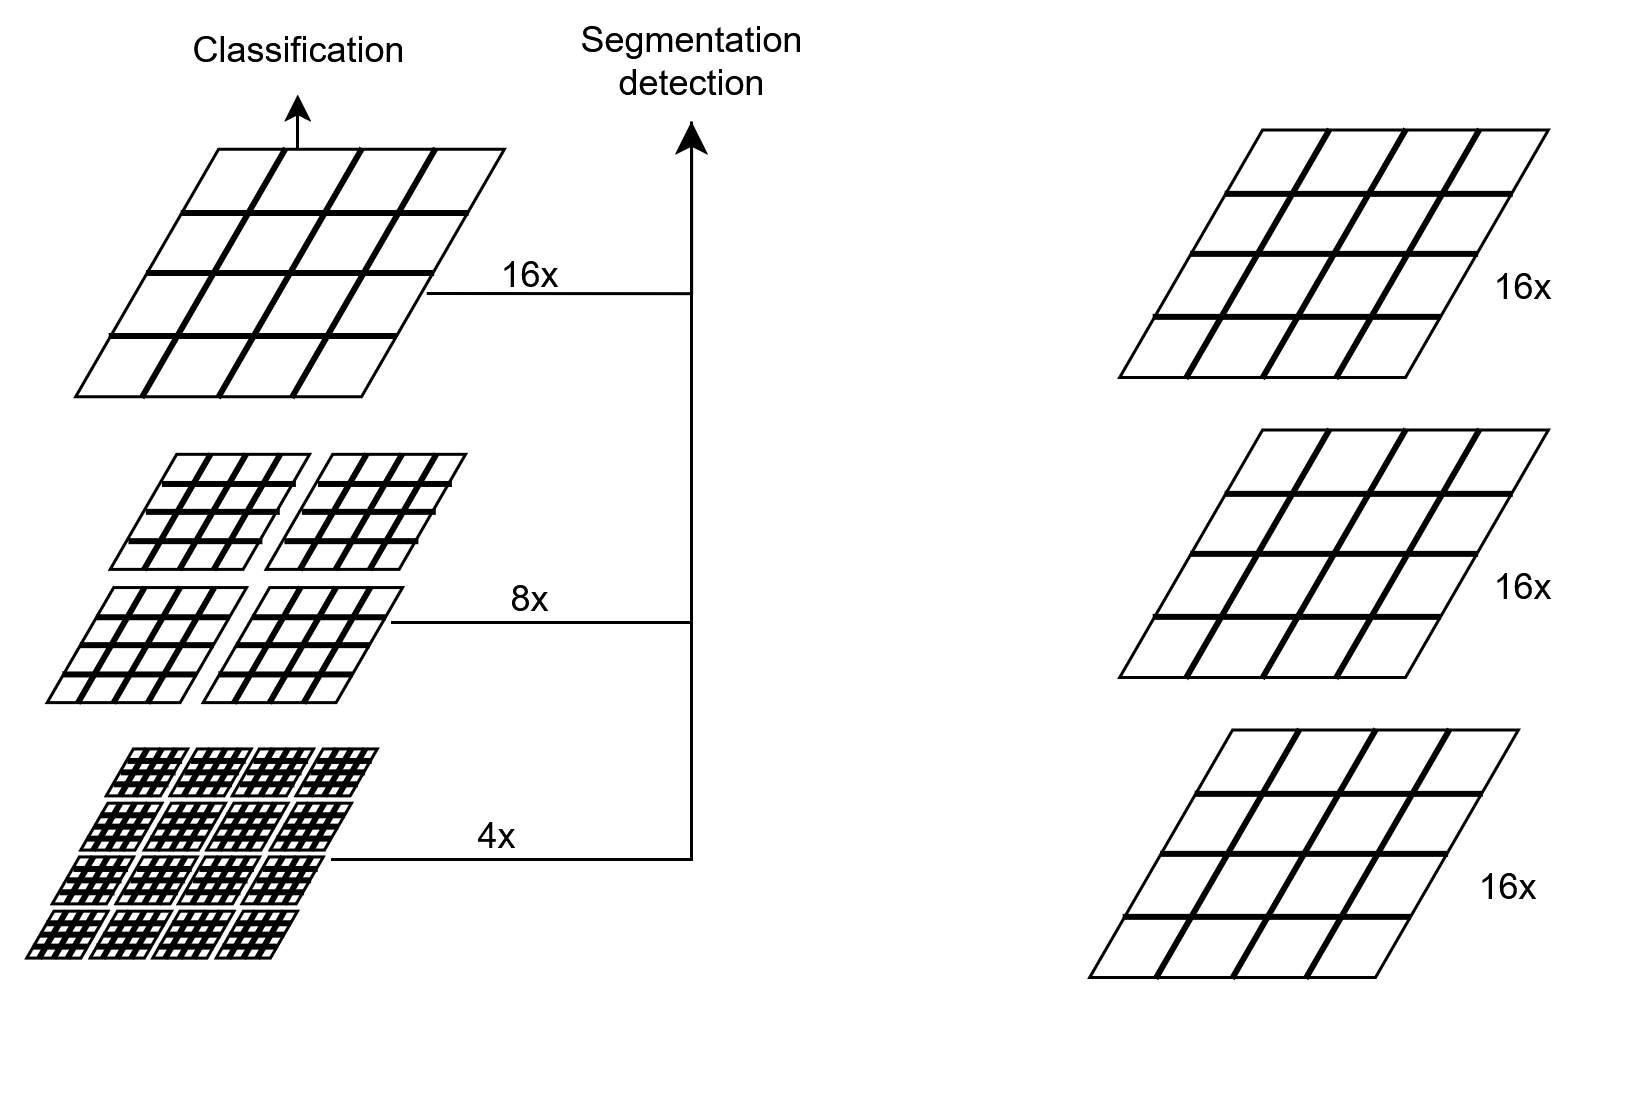
\includegraphics[width=0.8\textwidth]{images/swin-vit.png}
    \caption{Perbandingan antara \swin{} dan \vitfull{} \parencite{liu2021swin}.}
    \label{fig:Swin-vs-ViT}
\end{figure}


\autoref{fig:Swin-shifted-window} menujukkan pendekatan \shiftedwindow{} pada \swin. Selain itu, \swin{} mengadopsi arsitektur hierarkis yang mirip dengan \cnn. Arsitektur ini memungkinkan ekstraksi fitur pada berbagai skala dan menjadikannya lebih efisien dan fleksibel untuk menangani gambar resolusi tinggi dan berbagai tugas prediksi.

\begin{figure}[htbp]
    \centering
    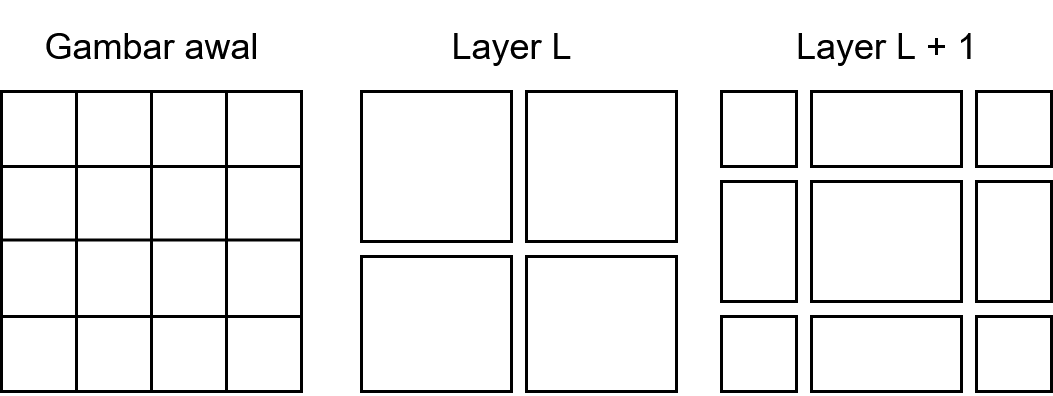
\includegraphics[width=0.7\textwidth]{images/swin-shifted-window.png}
    \caption{Pendekatan \shiftedwindow{} pada \swin{} \parencite{liu2021swin}.}
    \label{fig:Swin-shifted-window}
\end{figure}

Pada \swin, terdapat empat tahap. Pada setiap tahap, resolusi fitur akan secara bertahap dikurangi saat melalui lapisan \emph{patch merging} seperti pada \autoref{fig:swin-architecture}. Contohnya pada tahap satu, resolusi gambar $\frac{H}{4} \times \frac{W}{4}$ dengan dimensi fitur awal C. Kemudian pada tahap dua, resolusi dikurangi menjadi $\frac{H}{8} \times \frac{W}{8}$ dan 
dimensi fitur dinaikkan menjadi 2C. Tahap ini akan berlanjut hingga pada tahap empat dengan resolusi $\frac{H}{32} \times \frac{W}{32}$ dan dimensi 8C. Dengan struktur ini, \swin{} mampu menangkap informasi pada berbagai skala, seperti fitur lokal 
dan global, yang sangat penting dalam \emph{computer vision} seperti \emph{object detection}. 

\autoref{fig:swin-architecture} menunjukkan arsitektur dan cara kerja \swin. Gambar yang masuk dengan dimensi $H \times W$ akan dikonversi menjadi beberapa patch atau potongan kecil $4 \times 4$ pixel. Setiap \patch{} ini kemudian dianggap sebagai token, dan fitur awalnya direpresentasikan oleh nilai RGB-nya. Fitur ini kemudian 
diproyeksikan ke dimensi tertentu C melalui lapisan \emph{embedding} linier seperti yang ditunjukkan pada \autoref{fig:swin-architecture}.

\begin{figure}[htbp]
    \centering
    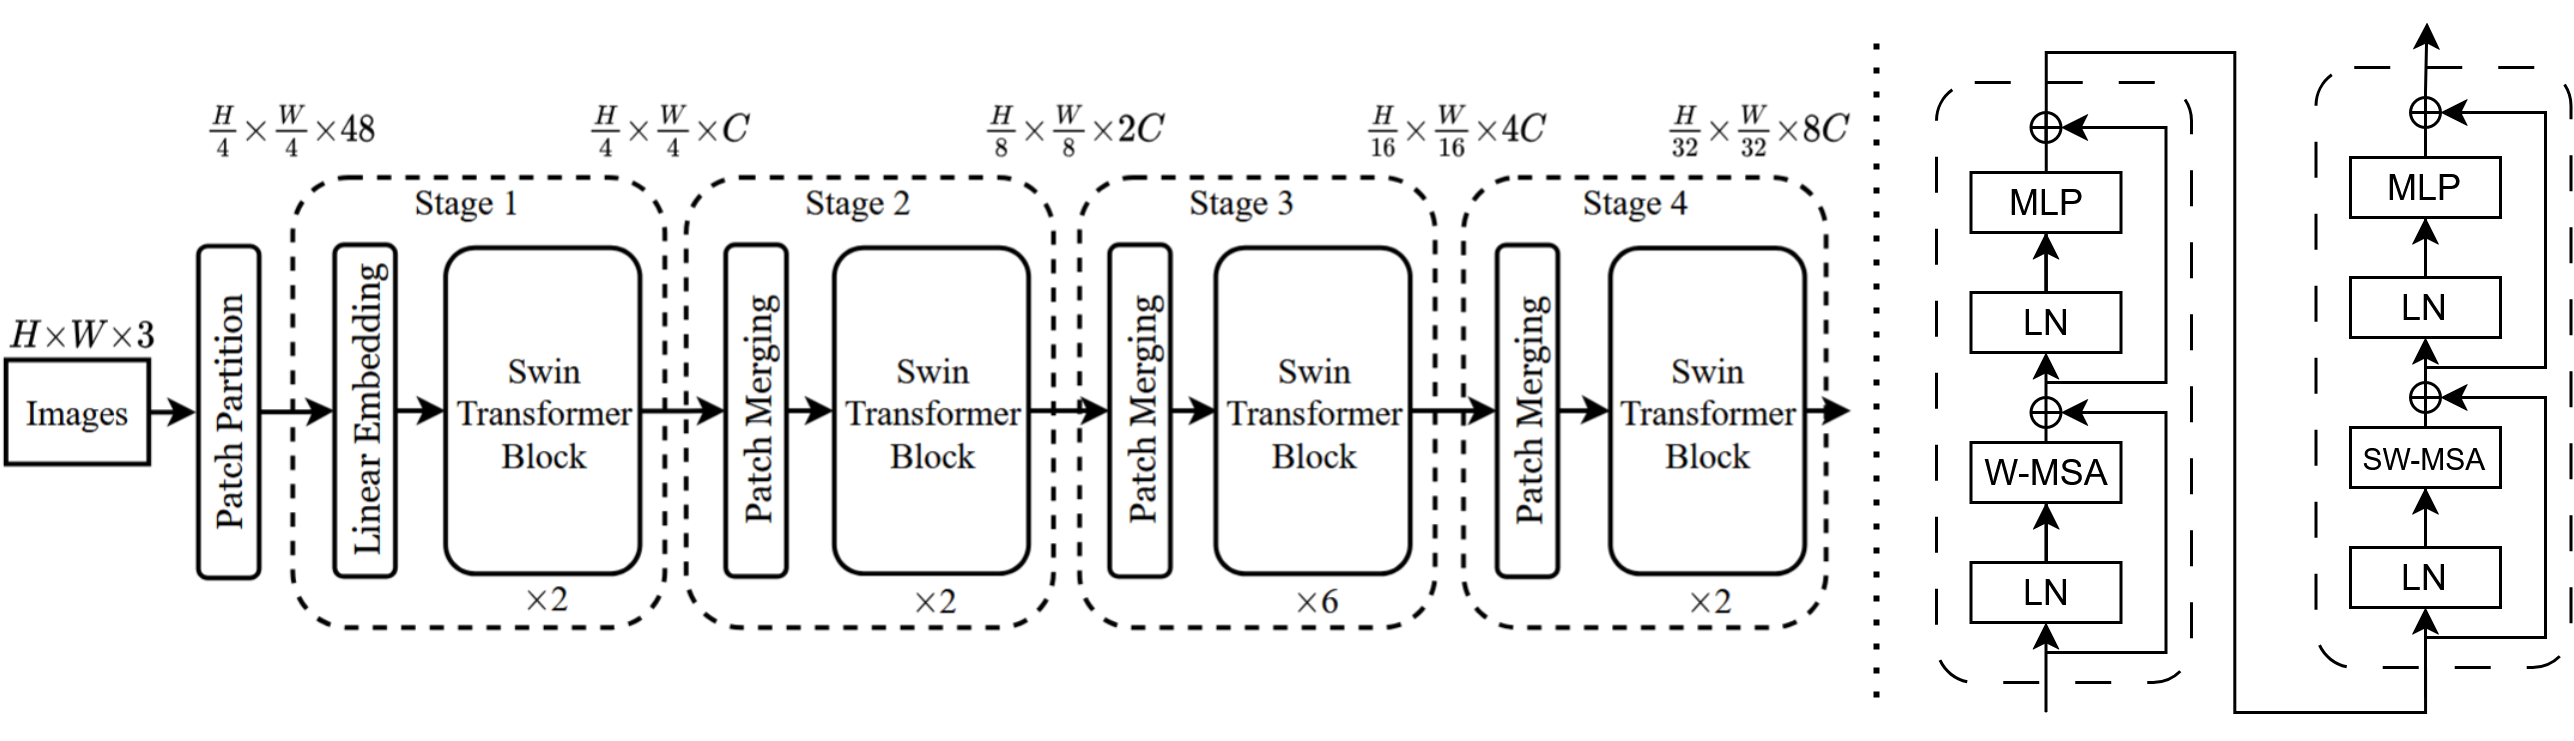
\includegraphics[width=1\textwidth]{images/swin-architecture.png}
    \caption{Arsitektur dan cara kerja \swin{} \parencite{liu2021swin}.}
    \label{fig:swin-architecture}
\end{figure}

\swin{} menggunakan \emph{Window Multi-Head Self-Attention} (W-MSA). Dengan metode ini, mekanisme \selfattention{} hanya dilakukan dalam \emph{window} lokal yang \emph{non-overlapping}. Contohnya ditunjukkan pada \autoref{fig:Swin-shifted-window}. 
Setiap \emph{window} memiliki ukuran $M \times M$ (umumnya $7 \times 7$) dan dengan membatasi \emph{attention} pada setiap \emph{window}, kompleksitas komputasi berkurang dari kuadratik menjadi linear terhadap ukuran gambar.

Untuk memungkinkan koneksi \emph{cross-window}, \swin{} 
menggunakan metode \emph{Shifted Window Multi-Head Self-Attention} (SW-MSA). 
Dalam metode ini, setiap window akan bergeser pada lapisan berikutnya dengan jarak tertentu (misalnya setengah ukuran jendela). Ini menciptakan koneksi cross window tanpa menambah banyak beban komputasi. Proses ini dapat dilihat pada \autoref{fig:Swin-shifted-window}. Window pada lapisan $l$ dan $l+1$ digeser untuk menciptakan interaksi 
satu sama lain. Dalam proses self-attention, Swin Transformer menggunakan \textit{relative position bias} untuk menangkap hubungan spasial antar \patch{}.


\subsection{\bartfull}
\label{subsec:bart}

\bartfull adalah adalah model \ml{} yang dirancang untuk memahami, menghasilkan, dan merekonstruksi teks dalam bahasa alami (\emph{natural language}). \bart{} merupakan \emph{denoising autoencoder} yang dilatih untuk memperbaiki teks yang telah "dirusak" (di-\emph{noise}) oleh berbagai transformasi sehingga mampu mengembalikan teks ke bentuk aslinya \parencite{lewis2019bart}. Arsitektur \bart{} menggabungkan kelebihan model \bert{} yang memiliki \emph{encoder bidirectional} dan GPT yang menggunakan \emph{decoder autoregressive}. Hal ini menjadikannya sangat fleksibel untuk berbagai tugas \nlpfull.

\bart{} dibangun di atas arsitektur transformer yang terdiri atas dua 
komponen utama, yaitu \emph{bidirectional encoder} dan \textit{autoregressive decoder}. 
\emph{Bidirectional encoder} akan mengolah teks input dengan cara memahami hubungan antar token secara dua arah. \emph{Autoregressive decoder} akan menghasilkan teks secara berurutan, token demi token, dengan mempertimbangkan \emph{sequence} yang sudah dihasilkan.

\begin{figure}
\centering
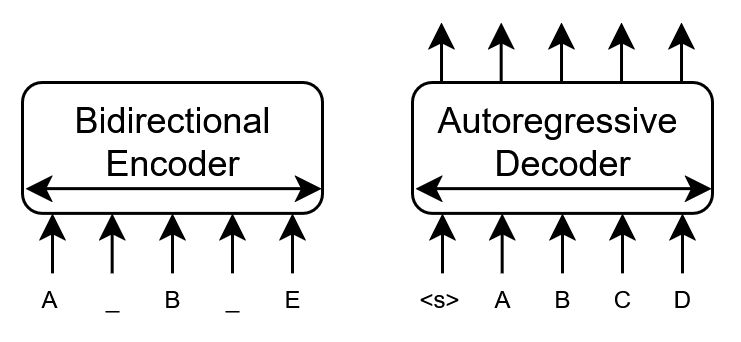
\includegraphics[width=0.8\textwidth]{images/bart.png}
\caption{Cara kerja \bart{} \parencite{lewis2019bart}.}
\label{fig:bart}
\end{figure}

\autoref{fig:bart} menunjukkan cara \bart{} bekerja. Teks input akan “dirusak” terlebih dahulu, kemudian dibaca oleh \encoder. Hasil bacaan \encoder{} akan diteruskan ke \decoder{} untuk mengembalikan bagian teks yang “dirusak” secara 
\textit{autoregressive}. Dengan kemampuannya untuk merekonstruksi teks dari masukan yang rusak, \bart{} menjadi suatu \transformer{} yang sangat baik untuk memahami struktur bahasa dan menghasilkan teks yang koheren walaupun masukan dinilai 
rusak. Penggunaan \bart{} mirip dengan \bert{} dan GPT, seperti klasifikasi teks, generasi teks, dan penejermahan teks. 




% \subsection{\onnx}
\label{subsec:onnx}

\emph{Open Neural Network Exchange} \onnx{} adalah format standar \emph{open-source} untuk merepresentasikan model \ml{} yang memungkinkan interoperabilitas antara berbagai \emph{framework} \dl. Dikembangkan oleh Facebook dan Microsoft pada tahun 2017, \onnx{} telah berkembang menjadi proyek yang lulus dari Linux Foundation AI dengan dukungan dari perusahaan teknologi besar termasuk IBM, Intel, AMD, ARM, Qualcomm, dan NVIDIA \parencite{onnxgithub2019}.

\onnx{} berfungsi sebagai representasi universal struktur komputasi dari \nn. Komponen arsitektur inti \onnx{} terdiri dari beberapa elemen penting. \emph{Node} merepresentasikan operasi matematika. \emph{Edge} merepresentasikan tensor yang mengalir antar operasi. \emph{Initializer} berfungsi untuk menyimpan bobot model dan konstanta yang diperlukan.

% Konsep teknis utama \onnx{} meliputi representasi menengah (\emph{Intermediate Representation}) yang berfungsi sebagai representasi universal untuk menangkap struktur graf komputasi dari jaringan neural. \onnx{} dibangun menggunakan format serialisasi \emph{Protocol Buffers} (protobuf) Google untuk penyimpanan dan transmisi model yang efisien. Format ini juga mendefinisikan \emph{Operator Set} (Opset) yang merupakan koleksi operator berversi untuk mempertahankan kompatibilitas mundur. Arsitektur \onnx{} merepresentasikan jaringan neural sebagai graf terarah asiklik (DAG) dimana \emph{node} merepresentasikan operasi dan \emph{edge} merepresentasikan aliran data.

% \subsubsection{Interoperabilitas dan Optimasi}

\onnx{} menyediakan interoperabilitas yang memungkinkan konversi model ke berbagai format, seperti \pytorch, \tensorflow, Keras, Scikit-learn, dan \emph{framework} lainnya. Hal ini memungkinkan \emph{deployment} tunggal yang memungkinkan pengembang untuk melakukan pelatihan model pada \emph{framework} apapun dan di-\emph{deploy} menggunakan \onnx Runtime. Format ini bersifat agnostik terhadap \emph{hardware} dan memungkinkan model berjalan di berbagai jenis \emph{hardware} seperti CPU, GPU, dan akselerator khusus seperti TPU.

% Dari aspek optimasi, \onnx{} menyediakan optimasi graf otomatis yang mencakup \emph{constant folding}, \emph{operator fusion}, dan eliminasi \emph{node} redundan. Format ini juga menyediakan optimasi spesifik \emph{hardware} yang memanfaatkan \emph{kernel} khusus untuk platform \emph{hardware} berbeda. Efisiensi memori juga menjadi keunggulan dengan alokasi memori yang dioptimalkan dan manajemen \emph{lifecycle} tensor yang efisien.

% \subsubsection{Aplikasi dalam \ml dan \cv}

% \onnx memiliki aplikasi luas dalam berbagai tugas \ml dan \cv. Dalam klasifikasi gambar, \onnx mendukung model seperti ResNet, EfficientNet, dan MobileNet untuk klasifikasi \emph{real-time}. Untuk deteksi objek, format ini kompatibel dengan model \yolo, SSD, dan \rcnn untuk berbagai aplikasi. Aplikasi lainnya mencakup segmentasi semantik dengan model U-Net dan DeepLab, sistem \ocr dan pemahaman dokumen untuk deteksi dan pengenalan teks, serta pengenalan wajah untuk sistem \emph{real-time} dan biometrik.

% Implementasi industri \onnx mencakup berbagai layanan besar seperti layanan Microsoft yang meliputi pencarian Bing, aplikasi Office, dan Azure Cognitive Services. Dalam industri otomotif, \onnx digunakan dalam sistem mengemudi otonom. Sektor kesehatan memanfaatkan \onnx untuk analisis pencitraan medis dan sistem diagnostik, sementara manufaktur menggunakannya untuk sistem kontrol kualitas dan deteksi cacat \parencite{onnxruntime2020}.


\subsection{\flutter}
\label{subsec:flutter}

\flutter{} adalah SDK (\emph{Software Development Kit}) UI \emph{open-source} dari Google yang diluncurkan pada tahun 2017. \flutter{} dirancang sebagai \emph{framework cross-platform} yang memungkinkan pengembang untuk membuat aplikasi yang dapat dijalankan secara \emph{native} pada berbagai \emph{platform} pada \emph{mobile}Berdasarkan standar penilaian yang kami buat, video UTS memberikan penjelasan yang sudah cukup lengkap, Pak. Tetapi, masih ada kekurangan minor dalam penjelasan jika dibandingkan dengan beberapa video lainnya seperti asumsi yang tidak disebutkan, visualisasi yang kurang menunjukkan tahapan pengerjaan dan perhitungan hasil. 

Nilai akhir mahasiswa yang berada pada 84.49 menunjukkan adanya kemungkinan mendapatkan nilai A pada batas 85. 
Jika terdapat pertimbangan untuk merubah penilaian, nilai UTS untuk soal 2 dapat diubah menjadi 4 dengan mempertimbangkan pemahaman pada soal 2 tentang Huffman Coding sebagai pemahaman yang sudah sangat baik. Kekurangan minor pada soal 2 karena adanya kekurangan visualisasi perhitungan yang terstruktur untuk mendapatkan hasil pengerjaan., \emph{web}, \emph{desktop}, dan perangkat \emph{embedded} dari satu \emph{codebase} \parencite{flutter2021}.

\flutter{} memiliki beberapa karakteristik utama yang membedakannya dari \emph{framework} pengembangan aplikasi lainnya, yaitu arsitektur \emph{single codebase} yang memungkinkan pengembangan \emph{cross-platform} dengan penulisan kode satu kali. Flutter juga menggunakan arsitektur berbasis \emph{widget}. Aristektur ini membuat segala sesuatu menjadi \emph{widget} yang merupakan komponen UI yang bersifat \emph{immutable}. 

% \flutter{} terdiri dari tiga \layer utama yang saling terintegrasi. \emph{Layer Framework} yang ditulis dalam Dart untuk implementasi desai \emph{platform-specific}. \emph{Layer widget} menyediakan abstraksi komposisi untuk membangun UI yang kompleks. \emph{layer rendering} menangani manajemen \emph{layout} dan posisi elemen. \emph{Layer foundation} menyediakan layanan inti seperti animasi, \emph{painting}, dan \emph{gestures} yang fundamental untuk interaksi pengguna.

% \emph{Layer Engine} yang ditulis dalam C++ berisi mesin grafis Skia untuk \emph{rendering} dengan transisi menuju Impeller untuk performa yang lebih baik. Runtime Dart dan \emph{virtual machine} berjalan pada layer ini untuk eksekusi kode aplikasi. \emph{Layout} teks dan operasi \emph{file} I/O juga dikelola pada layer ini, bersama dengan implementasi tingkat rendah dari \api inti \flutter.

% \emph{Layer Embedder} bersifat spesifik platform dan menangani integrasi dengan sistem operasi yang mendasarinya. Untuk Android menggunakan Java/C++, sedangkan iOS menggunakan Swift/Objective-C. Layer ini bertanggung jawab untuk koordinasi layanan sistem operasi, manajemen \emph{event loop}, dan eksposur \api spesifik platform untuk fungsionalitas yang tidak tersedia secara cross-platform.

% \subsubsection{\emph{Cross-Platform Development}}

\flutter{} menyediakan efisiensi pengembangan yang signifikan dibandingkan pengembangan tradisional. Pengembang dapat menargetkan \emph{multiple platform} secara bersamaan, mengurangi kebutuhan tenaga kerja dan kompleksitas manajemen proyek. Lingkungan pengembangan dan \emph{tools} yang terpadu memungkinkan konsistensi selama proses pengembangan.

% Konsistensi menjadi aspek penting dengan UI yang identik di semua platform, memberikan pengalaman pengguna yang seragam. Perilaku dan kinerja yang konsisten mengurangi bug spesifik platform dan memberikan pengalaman \emph{brand} yang terpadu. Hal ini sangat penting untuk aplikasi komersial yang memerlukan identitas visual yang kuat di berbagai platform.

% \subsubsection{Integrasi dengan \ml dan \cv}

\flutter{} menyediakan beberapa jalur untuk integrasi \ml{} yang relevan untuk aplikasi \cv{}. Integrasi \tensorflow Lite dengan \flutter{} didukung melalui paket \texttt{tflite\_flutter} yang memungkinkan inferensi model langsung pada perangkat. Implementasi dan inferensi dari model kustom dan \emph{pre-trained} juga didukung untuk kompatibilitas \emph{multi-platform}.

% Firebase ML Kit menyediakan \api ML \emph{on-device} untuk tugas umum seperti pengenalan teks, deteksi wajah, dan \emph{scanning barcode}. \emph{Labeling} gambar dan deteksi \emph{landmark} juga tersedia dengan kemampuan pemrosesan \emph{real-time} yang memadai untuk aplikasi produksi. Kemampuan \cv dalam \flutter mencakup pemrosesan \emph{stream} kamera \emph{real-time} untuk aplikasi yang memerlukan analisis video langsung. Klasifikasi gambar dan deteksi objek dapat diimplementasikan dengan mudah, begitu juga dengan implementasi \ocr untuk pengenalan teks. Pengenalan wajah dan autentikasi biometrik juga didukung untuk aplikasi keamanan \parencite{flutteronnx2022}.


\subsection{FastAPI}
\label{subsec:fastapi}

FastAPI adalah \emph{framework} \emph{web} Python modern dan berperforma tinggi untuk membangun \api{} dengan Python 3.7+ berdasarkan \emph{type hints} standar Python. Dibuat oleh Sebastián Ramírez, \emph{framework} ini merepresentasikan evolusi signifikan dalam pengembangan \emph{web} Python. FastAPI menggabungkan kesederhanaan Flask dengan kekuatan pemrograman \emph{asynchronous} modern \parencite{ramirez2020fastapi}.

FastAPI memiliki integrasi sistem \emph{type} sebagai fitur unggulan yang memanfaatkan sistem \emph{type hint} Python untuk validasi data otomatis, serialisasi, dan pembuatan dokumentasi secara otomatis. FastAPI memiliki \emph{tools} dokumentasi yang sudah terintegrasi, yaitu OpenAPI (sebelumnya Swagger). \emph{Framework} ini juga menggunakan skema \json yang memberikan kompatibilitas yang luas dengan ekosistem pengembangan modern. FastAPI dibangun di atas \emph{Asynchronous Server Gateway Interface} (ASGI) yang mewakili kemajuan arsitektur yang signifikan dibandingkan \emph{framework} berbasis \emph{Web Server Gateway Interface} (WSGI) tradisional \parencite{ramirez2020fastapi}. 

% Komponen arsitektur ASGI meliputi \emph{scope} yang berisi informasi \emph{scope} koneksi dengan tipe protokol dan metadata yang diperlukan. \emph{Receive} berfungsi sebagai \emph{callable awaitable} untuk menerima \emph{event} dari \emph{client}, sementara \emph{send} bertindak sebagai \emph{callable awaitable} untuk mengirim respons ke \emph{client}.

% Arsitektur berlapis FastAPI terdiri dari beberapa \layer terintegrasi yang bekerja secara harmonis. \emph{Application Layer} merupakan aplikasi inti FastAPI yang menangani \emph{routing} dan \emph{dependency injection} dengan sistem yang sophisticated. \emph{Framework Layer} menggunakan Starlette yang menyediakan kompatibilitas ASGI dan fungsionalitas \emph{framework} web yang diperlukan. \emph{Validation Layer} memanfaatkan Pydantic untuk validasi dan serialisasi data dengan performa tinggi, sementara \emph{Server Layer} menggunakan \emph{server} ASGI Uvicorn untuk penanganan \emph{request} HTTP yang efisien.

% \subsubsection{\emph{Async Programming} dan Kinerja}

% Model \emph{async processing} membedakan FastAPI dari \emph{framework synchronous} tradisional dengan memproses \emph{request} secara asinkron. \emph{Event loop single-threaded} menangani berbagai koneksi bersamaan tanpa overhead context switching yang tinggi. \emph{Coroutines} memungkinkan fungsi \emph{async} yang dapat dihentikan dan dilanjutkan sesuai kebutuhan, sementara \emph{non-blocking} I/O memberikan penanganan operasi I/O yang efisien tanpa memblokir \emph{thread} utama.

% Analisis kinerja berdasarkan \emph{benchmark} TechEmpower independen menunjukkan kinerja superior FastAPI dalam berbagai aspek. \emph{Throughput} FastAPI mencapai sekitar 3 kali lebih tinggi dari Flask dalam kondisi beban tinggi. P99 \emph{latency} yang lebih rendah dicapai karena pemrosesan \emph{async} yang efisien, sementara efisiensi memori menunjukkan \emph{footprint} memori yang berkurang per \emph{request}. Karakteristik \emph{scaling} linear dengan \emph{concurrent requests} memungkinkan aplikasi menangani beban yang meningkat dengan graceful degradation.

% \subsubsection{Integrasi dengan Sistem \cv dan \ml}

% FastAPI menyediakan arsitektur optimal untuk \emph{deployment} model \ml dalam konteks \cv dengan berbagai kemampuan teknis. Pemrosesan \emph{async} memungkinkan pemrosesan gambar \emph{non-blocking} untuk \emph{throughput} tinggi, sangat penting untuk aplikasi yang menangani volume gambar besar. Manajemen memori yang efisien memungkinkan penanganan data gambar besar tanpa degradasi performa yang signifikan. Dukungan \emph{streaming} memungkinkan kemampuan pemrosesan video \emph{real-time} untuk aplikasi yang memerlukan analisis kontinyu, sementara pemrosesan bersamaan memungkinkan \emph{multiple pipeline} pemrosesan gambar berjalan secara paralel.

% Arsitektur \emph{model serving} yang disediakan FastAPI mencakup tahapan yang komprehensif. \emph{Model loading} terjadi saat \emph{startup} aplikasi untuk memuat model \ml ke memori dengan efisien. \emph{Preprocessing pipeline} menangani tahap preprocessing gambar sebelum inferensi untuk memastikan format data yang sesuai. Inferensi model dilakukan dengan eksekusi model \ml untuk prediksi yang akurat dan cepat. \emph{Postprocessing} memproses hasil prediksi untuk format yang diinginkan sesuai kebutuhan aplikasi, dan \emph{response serialization} melakukan serialisasi hasil ke format \json atau format lainnya sesuai spesifikasi \api.

% FastAPI mendukung integrasi dengan berbagai \emph{library} \ml Python seperti \pytorch, \tensorflow, dan \onnx Runtime, menjadikannya pilihan yang sesuai untuk \emph{deployment} model \cv dalam lingkungan produksi \parencite{techempowerbenchmark2023}.


\subsection{Metrik Evaluasi}
\label{subsec:metrik-evaluasi}

Evaluasi kinerja sistem \ml{} memerlukan metrik yang komprehensif dan sesuai dengan domain aplikasi. Sistem pemahaman dokumen dan pengenalan teks memerlukan kombinasi metrik klasifikasi standar dan metrik khusus untuk evaluasi pemahaman dokumen. Metrik evaluasi yang digunakan dalam penelitian ini mencakup \accuracy, \precision, \recall, \fscore, \coverage, dan \mcer{} (\emph{Mean Character Error Rate}).

\subsubsection{Metrik Klasifikasi Standar}

\accuracyfl{} mengukur proporsi prediksi yang benar baik positif maupun negatif di seluruh \emph{instance} dalam \dataset. Formula \accuracy{} didefinisikan sebagai perbandingan antara jumlah prediksi benar dengan total prediksi yang dibuat. Dalam konteks klasifikasi biner, \accuracy{} dihitung menggunakan matriks yang terdiri dari \emph{True Positive} (TP), \emph{True Negative} (TN), \emph{False Positive} (FP), dan \emph{False Negative} (FN). Persamaan \eqref{eq:accuracy} menunjukkan perhitungan \accuracy{} \parencite{jayaswal2020evalmetrics}. 

\begin{equation}
    \label{eq:accuracy}
\text{Accuracy} = \frac{TP + TN}{TP + TN + FP + FN}
\end{equation}

\precisionfl{} mengukur proporsi prediksi positif yang benar di antara semua prediksi positif yang dibuat model. Metrik ini sangat penting ketika biaya \emph{false positive} tinggi dalam aplikasi tertentu. Persamaan \eqref{eq:precision} menunjukkan perhitungan \precision. Perhitungan \precision{} didefinisikan sebagai rasio antara \emph{True Positive} (TP) dengan jumlah total prediksi positif yang dibuat, yaitu jumlah \emph{True Positive} ditambah \emph{False Positive} \parencite{jayaswal2020evalmetrics}. \precisionfl{} tinggi menunjukkan bahwa model meminimalkan \emph{false positive}, memastikan prediksi positif kemungkinan besar benar dan dapat diandalkan untuk pengambilan keputusan.

\begin{equation}
    \label{eq:precision}
\text{Precision} = \frac{TP}{TP + FP}
\end{equation}

\recallfl{} mengukur proporsi \emph{instance} positif aktual yang berhasil diidentifikasi dengan benar oleh model. Metrik ini kritikal ketika biaya \emph{false negative} tinggi dalam sistem yang memerlukan deteksi lengkap. Persamaan \eqref{eq:recall} menunjukkan rumus yang dapat digunakan untuk menghitung \recall{} \parencite{jayaswal2020evalmetrics}.\recallfl{} tinggi berarti model menangkap sebagian besar \emph{instance} positif, meminimalkan kemungkinan melewatkan data penting yang harus dideteksi.

\begin{equation}
    \label{eq:recall}
\text{Recall} = \frac{TP}{TP + FN}
\end{equation}

\fscore{} adalah rata-rata harmonik dari \precision{} dan \recall{}. \fscore{} memberikan ukuran seimbang yang mempertimbangkan kedua metrik secara setara. Persamaan \eqref{eq:fscore} menunjukkan rumus yang dapat digunakan untuk menghitung \fscore{} \parencite{jayaswal2020evalmetrics}. \fscore{} tinggi menunjukkan bahwa model tidak hanya akurat dalam prediksi positif tetapi juga menangkap sebagian besar \emph{instance} positif yang relevan. \fscore{} memerlukan \precision{} dan \recall{} tinggi untuk mencapai skor tinggi. \fscore{} akan menjadi nol jika salah satu dari \precision{} atau \recall{} adalah nol.

\begin{equation}
    \label{eq:fscore}
\text{F1-Score} = 2 \times \frac{\text{Precision} \times \text{Recall}}{\text{Precision} + \text{Recall}}
\end{equation}

% \subsubsection{\ted (\emph{Tree Edit Distance})}

\ted adalah \emph{sequence minimum-cost} dari operasi edit \emph{node} yang diperlukan untuk mentransformasi satu \emph{tree} menjadi \emph{tree} lain \parencite{zhang1989tree}. Operasi edit yang dapat dilakukan meliputi \emph{delete} untuk menghapus \emph{node} dan menghubungkan \emph{children}-nya ke \emph{parent}, \emph{insert} untuk menambahkan \emph{node} antara \emph{node} yang ada dan \emph{children}-nya, dan \emph{relabel} untuk mengubah \emph{label} dari \emph{node}.

Formulasi matematika \ted didefinisikan sebagai optimasi biaya minimum untuk transformasi struktur \emph{tree}.

\begin{equation}
\text{TED}(T_1, T_2) = \min\{\text{cost}(\text{sequence}) : \text{sequence transforms } T_1 \text{ to } T_2\}
\end{equation}

Definisi rekursif \ted memungkinkan perhitungan efisien melalui pemrograman dinamis.

\begin{equation}
\text{TED}(F, G) = \min \begin{cases}
\text{TED}(F-v, G) + \text{cost}(\text{delete } v) \\
\text{TED}(F, G-w) + \text{cost}(\text{insert } w) \\
\text{TED}(F-v, G-w) + \text{cost}(\text{relabel } v \rightarrow w)
\end{cases}
\end{equation}

\ted memiliki aplikasi luas dalam pemahaman dokumen terstruktur, mencakup analisis similaritas dokumen XML/HTML, analisis dan perbandingan \emph{layout} dokumen, pengenalan struktur dokumen yang kompleks, dan perbandingan data hierarkis. Dalam konteks pemahaman dokumen, \ted berguna untuk mengevaluasi seberapa baik model memahami struktur hierarkis informasi dalam dokumen terstruktur.

\subsubsection{\mcer{} (\emph{Mean Character Error Rate})}

\mcer{} adalah rata-rata \emph{Character Error Rate} (CER) di beberapa dokumen atau segmen teks yang memberikan ukuran komprehensif akurasi deteksi teks \parencite{holley2009ocr}. Metrik ini sangat relevan untuk sistem pengenalan teks yang bergantung pada akurasi pengenalan karakter. Persamaan \eqref{eq:mcer} menunjukkan rumus yang digunakan untuk menghitung \mcer dengan $\text{CER}_i$ adalah \emph{Character Error Rate} untuk dokumen $i$. Metrik ini mengukur kesalahan pengenalan karakter pada tingkat granular dan memberikan informasi tentang akurasi pengenalan teks pada level karakter.

\begin{equation}
    \label{eq:mcer}
\text{mCER} = \frac{1}{N} \times \sum_{i=1}^{N} \text{CER}_i
\end{equation}

\begin{equation}
    \label{eq:cer}
\text{CER}_i = \frac{S_i + D_i + I_i}{N_i}
\end{equation}

Persamaan \eqref{eq:cer} menunjukkan cara perhitungan CER dengan parameter yang meliputi $S$ yang merepresentasikan jumlah substitusi karakter, $D$ untuk jumlah \emph{deletion} atau penghapusan karakter, $I$ untuk jumlah \emph{insertion} atau penambahan karakter, dan $N$ sebagai total jumlah karakter dalam \emph{ground truth}.

% \mcer{} digunakan secara luas dalam berbagai aplikasi evaluasi \ocr. \emph{Benchmark} mesin \ocr{} menggunakan \mcer{} untuk membandingkan kinerja algoritma yang berbeda dan memantau perkembangan dari waktu ke waktu. Proyek digitalisasi menggunakan metrik ini untuk menilai kualitas hasil konversi dokumen fisik ke digital.

% \subsubsection{Integrasi Metrik untuk Evaluasi Sistem}

% Evaluasi sistem pemahaman dokumen yang komprehensif memerlukan pendekatan \emph{multi-level} yang mengintegrasikan berbagai metrik. Tingkat karakter menggunakan \mcer untuk mengukur akurasi pengenalan teks individual dan memastikan setiap karakter dapat dibaca dengan benar. Tingkat \emph{field} memanfaatkan \accuracy, \precision, \recall, dan F1-\emph{score} untuk evaluasi ekstraksi \emph{field} spesifik dalam dokumen terstruktur. Tingkat struktur menggunakan \ted untuk mengevaluasi pemahaman struktur dokumen keseluruhan dan hubungan antar elemen. Tingkat sistem mengkombinasikan semua metrik untuk evaluasi kinerja sistem secara holistik.

% Interpretasi dan \emph{trade-off} antar metrik memberikan perspektif berbeda tentang kinerja sistem. \accuracy memberikan gambaran umum kinerja tetapi dapat menyesatkan pada data tidak seimbang, sehingga perlu dikombinasikan dengan metrik lain. \precision menjadi penting ketika biaya \emph{false positive} tinggi dalam aplikasi yang memerlukan presisi tinggi. \recall kritikal ketika biaya \emph{false negative} tinggi dalam sistem yang memerlukan deteksi lengkap. F1-\emph{score} memberikan keseimbangan antara \precision dan \recall untuk evaluasi menyeluruh. \ted mengukur pemahaman struktur dokumen yang kompleks dan hubungan hierarkis antar elemen, sementara \mcer memberikan ukuran granular akurasi pengenalan teks pada level karakter.

% Penggunaan metrik evaluasi yang komprehensif memastikan bahwa sistem pemahaman dokumen tidak hanya akurat dalam mengenali teks, tetapi juga mampu memahami struktur dokumen dan mengekstrak informasi relevan dengan presisi tinggi yang diperlukan untuk berbagai aplikasi \parencite{bille2005tree}.

\subsubsection{\emph{System Usability Scale} (SUS)}
\label{subsubsec:sus}




\section{Penelitian Terkait}
\label{sec:penelitianterkait}

Subbab penelitian terkait akan memberikan rangkuman dari penelitian-penelitian yang pernah dilakukan pada kasus yang serupa atau menggunakan alternatif solusi yang serupa. Subbab ini ditujukan sebagai referensi untuk mendapatkan penggunaan alternatif solusi atau pendekatan yang telah dilakukan  terhadap masalah serupa. Berikut adalah penelitian-penelitian terkait tersebut. 

\subsection{\textit{A Comprehensive Analysis of LayoutLM and Donut for Document Classification}}
\label{sec:penelitian-1}
Penelitian oleh \textciteyear{bajrami2023comprehensive}  akan melakukan analisis komparasi dari dua buah \textit{pre-trained model} berbasis \transformer{}, yaitu \layoutlm{} dan \donut, untuk klasifikasi dokumen. Penelitian ini melakukan perbandingan kinerja kedua model pada dua \dataset{} dengan karakteristik berbeda dengan melakukan evaluasi 
terhadap nilai \accuracy, \precision, dan \fscore{} dari kedua model. 

\subsubsection{Gambaran Umum}
Penelitian ini bertujuan untuk membandingkan kinerja \donut{} dan \layoutlm{} dalam klasifikasi dokumen. Studi ini membandingkan kinerja keduanya pada data yang tidak terstuktur (\textit{unstructured data}), seperti struk, \textit{invoice}, dan catatan tulis tangan.

\subsubsection{Analisis dan Metode}
\layoutlm{} adalah model yang mengombinasikan deteksi objek, pengenalan teks, dan analisis \textit{layout}. \layoutlm{} memiliki dependensi terhadap teknologi \ocr{} untuk melakukan ekstraksi teks dari dokumen berbentuk gambar. \donut{} adalah sebuah model \transformer{} untuk melakukan pemahaman dokumen yang telah bersifat \sotafull{} dan tidak memerlukan integrasi \ocr{}.

Analisis komparasi kedua model ini dilakukan pada dua jenis \dataset. \datasetfl{} pertama adalah sebuah \dataset{} dengan jumlah 10.000 sampel data yang terdiri dari dokumen perusahaan dengan kompleksitas yang lebih tinggi. Dataset 
kedua terdiri dari 50.000 sampel yang lebih terdiversifikasi. Kedua model di-\textit{fine-tuned} dengan menggunakan \textit{transfer learning} dengan \textit{pre-trained weights} dan evaluasi dilakukan dengan metrik \accuracy, \precision, dan \fscore.  

Pada \dataset{} 1, hasil yang didapatkan dari model \layoutlm{} memiliki angka yang lebih tinggi, yaitu pada angka 0,88 dibandingkan dengan penggunaan model \donut{} pada angka 0,74. Hal ini mengindikasikan bahwa \layoutlm{} lebih unggul untuk menangani dokumen dengan struktur yang lebih kompleks dibandingkan \donut{}. Pada \dataset{} 2, \donut{} memiliki angka akurasi yang lebih tinggi, yaitu 0,91 sedangkan \layoutlm{} dengan mendapatkan angka 0,82 \parencite{bajrami2023comprehensive}.

\subsubsection{Kesimpulan}

\layoutlm{} dan \donut{} merupakan pilihan yang efektif untuk melakukan klasifikasi dokumen, tetapi dengan kebutuhan yang berbeda. \layoutlm{} lebih 
cocok untuk digunakan pada dokumen dengan kompleksitas yang lebih tinggi, namun hasil yang didapatkan lebih lama karena memiliki \textit{pipeline} yang lebih 
panjang akibat adanya proses \ocr{} terlebih dahulu. \donut{} lebih cocok untuk digunakan pada \dataset{} dengan diversifikasi dokumen yang lebih banyak dan dapat menghasilkan dengan lebih cepat akibat \emph{pipeline} yang lebih pendek akibat tidak perlu integrasi dengan \ocr. Dokumen yang memiliki \textit{noise} atau resolusi yang buruk akan mengurangi akurasi secara signifikan untuk \layoutlm{} dan \donut.
\subsection{\textit{An End-to-End OCR-Free Solution for Identity Document \linebreak Understanding}}
\label{sec:penelitian-2}
Penelitian yang dilakukan oleh \textciteyear{carta2024end}  menunjukkan penggunaan model \donut{} untuk melakukan ekstraksi data dari dokumen identitas. Dokumen yang digunakan dapat berupa kartu identitas elektronik, kartu identitas, surat izin 
mengemudi, dan kartu kesehatan. Evaluasi dilakukan dengan membandingkan model yang telah mengalami proses \textit{fine-tuning} dan model basis yang ada dengan mempertimbangkan faktor \fscore, \mcerfull, \tedfull. 

\subsubsection{Gambaran Umum}
Sebuah penelitian oleh \textciteyear{carta2024end} mempresentasikan hasil implementasi \donut{} untuk pengenalan dokumen identitas. Tujuan utama dari penelitian ini adalah menyediakan solusi untuk menjawab tantangan dalam melakukan ekstraksi dan verifikasi data dokumen identitas secara manual pada servis digital. Penelitian ini menggunakan teknologi terbaru pada \textit{Document Understanding} (DU) dan \ml{} untuk otomasi pengenalan dokumen identitas. Solusi yang digunakan menggunakan proses \textit{fine-tuning} dua tahap, yaitu model \textit{pre-trained} dan pelatihan pada \dataset{} sintetis dan asli. Hal ini dilakukan dengan tujuan untuk mengekstrak informasi dari kartu identitas secara efisien. Selama pengembangan, terdapat isu seperti data asli yang terbatas, kualitas gambar yang buruk, dan format identitas yang beragam. 

\subsubsection{Analisis dan Metode}
Solusi yang ditawarkan menggunakan arsitektur \transformer{} \donut{} yang mengutilisasi \swin{} sebagai \encoder{} dan BART sebagai \decoder{}. Arsitektur ini memberikan implementasi yang bebas dari \ocr{} untuk ekstraksi teks dan pemahaman \emph{layout}. Walaupun \donut{} adalah \textit{pre-trained model}, \donut{} tetap memerlukan dataset yang besar untuk melalui proses \emph{fine-tuning}. Terdapat dua fase \emph{fine-tuning} yang dilakukan, yaitu \emph{fine-tuning} dengan data sintetis dengan format, konten, dan \emph{layout} bervariasi dan \emph{fine-tuning} dengan data dokumen identitas asli untuk meningkatkan akurasi solusi yang ditawarkan. Dokumen identitas yang digunakan terdiri dari \emph{Electronic ID Card} (EIC), \emph{Identity Card} (IC), \emph{Health Card} (HC), dan \emph{Driving License} (DL). Evaluasi terhadap solusi dilakukan dengan menggunakan metrik \fscore, \mcerfull, dan \tedfull. Eksperimen dilakukan pada 20\% \emph{test data} dan 80\% \emph{train data} dengan hasil perbandingan implementasi \donut{} sebelum dan setelah \textit{fine-tuning} disajikan pada \autoref{tab:donut-comparison-on-id-documents}. 

\begin{table}[h!]
    \centering % Centers the table on the page
    \caption{Hasil perbandingan implementasi Donut sebelum dan setelah \textit{fine-tuning} \parencite{carta2024end}.}
    \label{tab:donut-comparison-on-id-documents}
    \begin{tabularx}{\textwidth}{|X|C|C|C|C|C|C|}
        \hline
        % --- First Header Row ---
        % The "Dokumen" cell spans 2 rows vertically.
        % The "Donut Base" and "Donut Synth" cells each span 3 columns horizontally.
        \multirow{2}{*}{Dokumen} & \multicolumn{3}{c|}{Donut Base} & \multicolumn{3}{c|}{Donut Synth} \\
        \cline{2-7} % Creates a horizontal line from column 2 to 7
        
        % --- Second Header Row ---
        % The first column is left blank because the multirow cell is occupying it.
        & TED & F1 & mCER & TED & F1 & mCER \\
        \hline% Double line to separate header from body
        
        % --- Table Body ---
        EIC & 0.821 & 0.441 & 0.136 & 0.893 & 0.554 & 0.084 \\ \hline
        IC  & 0.769 & 0.594 & 0.171 & 0.885 & 0.712 & 0.090 \\ \hline
        HC  & 0.959 & 0.891 & 0.039 & 0.986 & 0.943 & 0.014 \\ \hline
        DL  & 0.929 & 0.813 & 0.057 & 0.973 & 0.866 & 0.025 \\ \hline
    \end{tabularx}
\end{table}

\subsubsection{Kesimpulan}
Implementasi solusi dengan menggunakan arsitektur \donut{} dapat  melakukan ekstraksi informasi secara akurat dari dokumen identitas tanpa memerlukan implementasi \ocr{} yang konvensional. Proses \textit{fine-tuning} dua tahap sangat direkomendasikan karena ketersediaan data asli yang terbatas \parencite{carta2024end}. Eksperimen yang dilakukan mengonfirmasi proses \textit{fine-tuning} akan meningkatkan performa dari \emph{base model}.  
\subsection{\textit{The Future of Document Indexing: GPT and Donut Revolutionize Table of Content Processing}}
\label{sec:penelitian-3}
Penelitian yang dilakukan oleh \textciteyear{feyisa2024future} ini mempresentasikan bagaimana model dengan arsitektur \donut{} dan GPT-3.5 Turbo dapat digunakan untuk melakukan ekstraksi informasi dari dokumen tanpa perlu adanya pendekatan manual yang dilakukan. Dokumen yang digunakan merupakan data yang terstruktur dan bersifat kompleks. Hasil dari model yang digunakan disajikan dalam bentuk 
\textit{dashboard} dan dievaluasi dengan menggunakan akurasi setiap model yang digunakan.

\subsubsection{Gambaran Umum}
Penelitian ini menjelaskan mengenai bagaimana teknologi AI seperti \donut{} dan GPT-3.5 Turbo membuat gebrakan baru pada pemrosesan \emph{document indexing} dan daftar isi untuk dokumen-dokumen kompleks. Permasalahan yang ditemukan adalah ekstraksi informasi secara manual dari dokumen yang kompleks dan panjang sangat memakan waktu dan rawan kesalahan. 

\subsubsection{Analisis dan Metode}
Solusi yang digunakan adalah solusi berbasis AI dengan menggunakan model dengan arsitektur \donut{} untuk melakukan ekstraksi data dari gambar dan dokumen dan GPT-3.5 Turbo untuk melakukan retrukturisasi daftar isi. Sistem yang dirancang akan mengidentifikasi halaman daftar isi dan melakukan ekstraksi \emph{headings} dan \emph{subheadings}-nya dan mengonversinya menjadi data dengan format \json{} yang terstruktur untuk digunakan pada \emph{dashboard} atau \emph{database}.  

Data atau dokumen yang digunakan akan dikonversi menjadi gambar untuk 
\donut{} dan teks untuk GPT untuk kemudian digunakan untuk melakukan \emph{fine-tuning} model pada fase \emph{training model} \parencite{feyisa2024future}. Model yang telah di-\emph{fine-tune} ini akan melakukan identifikasi halaman daftar isi dan melakukan ekstraksi dan merestrukturisasi \emph{headings} dan \emph{subheadings} dalam format \json. Hasil yang telah diekstrak dalam format \json{} akan diintegrasikan ke dalam \emph{dashboard} yang telah dibuat dalam bentuk \emph{website}. Evaluasi terhadap model dilakukan dengan 
menggunakan \accuracy{}. Model dengan arsitektur Donut yang digunakan mencapai nilai \accuracy{} hingga 85\% dan GPT-3.5 Turbo mencapai \accuracy{} 89\%. 

\subsubsection{Kesimpulan}

Penggunaan \emph{Large Language Model} (LLM) dan teknologi \cv, seperti OpenAI GPT-3.5 Turbo dan \donut, memberikan solusi yang efisien untuk menyusun informasi dari dokumen besar secara otomatis. Dengan kemampuan untuk mengorganisasi data, seperti daftar isi dalam dokumen spesifikasi, teknologi ini mampu mengurangi risiko kesalahan, waktu, dan biaya yang berlebihan. 
% Pendekatan ini menjadi langkah inovatif yang mendukung pengelolaan dokumen teknis yang kompleks dan meningkatkan efisiensi dan akurasi dalam berbagai sektor industri. 

\subsection{Contoh Bikin Equation}
\textbf{text tebal} dan ini \emph{miring}, bikin persamaan di baris yang sama, tinggal pake dolar2 $\Psi(\vec{r}_1,...,\vec{r}_N)$, sehingga persamaan Schr\"{o}dinger, terus, persamaan yang dinomeri kayak gini
%ini contoh bikin persamaan, ..... :D
\begin{equation}
	\left[ \sum_{i}^{N}-\frac{\hbar^2}{2m}\nabla_i^2 + \sum_{i}^{N}V(\vec{r}_i)+ \sum_{i<j}^{N}(\vec{r}_i,\vec{r}_j)\right]\Psi = E\Psi
\end{equation}

untuk $N$-elektron, dengan $\hat{H}$=Hamiltonian, $E$=Energi total, $\hat{T}$=Energi kinetik, $\hat{V}$=Energi potensial, dan $\hat{U}$=Interaksi ektron-elektron.

\subsection{Bikin Matrix}
Lalalallala.... bikin matrix sekarang, yang ini dikecilin, pake smaller
	{\smaller
		\begin{equation}
			\Psi({\bf r}_1, {\bf r}_2, \cdots {\bf r}_N) = \frac{1}{\sqrt{N!}}\left| \begin{array}{llcl}
				\phi_1({\bf r}_1)     & \phi_2({\bf r}_1)     & \cdots                & \phi_N({\bf r}_1)     \\
				\phi_1({\bf r}_2)     & \phi_2({\bf r}_2)     & \cdots                & \phi_N({\bf r}_2)     \\
				\phi_1({\bf r}_3)     & \phi_2({\bf r}_3)     & \cdots                & \phi_N({\bf r}_3)     \\
				\multicolumn{1}{c}{.} & \multicolumn{1}{c}{.} & \multicolumn{1}{c}{.} & \multicolumn{1}{c}{.} \\
				\multicolumn{1}{c}{.} & \multicolumn{1}{c}{.} & \multicolumn{1}{c}{.} & \multicolumn{1}{c}{.} \\
				\multicolumn{1}{c}{.} & \multicolumn{1}{c}{.} & \multicolumn{1}{c}{.} & \multicolumn{1}{c}{.} \\
				\phi_1({\bf r}_N)     & \phi_2({\bf r}_N)     & \cdots                & \phi_N({\bf r}_N)     \\
			\end{array} \right|
		\end{equation}
	}